% This is the Reed College LaTeX thesis template. Most of the work 
% for the document class was done by Sam Noble (SN), as well as this
% template. Later comments etc. by Ben Salzberg (BTS). Additional
% restructuring and APA support by Jess Youngberg (JY).
% Your comments and suggestions are more than welcome; please email
% them to cus@reed.edu
%
% See http://web.reed.edu/cis/help/latex.html for help. There are a 
% great bunch of help pages there, with notes on
% getting started, bibtex, etc. Go there and read it if you're not
% already familiar with LaTeX.
%
% Any line that starts with a percent symbol is a comment. 
% They won't show up in the document, and are useful for notes 
% to yourself and explaining commands. 
% Commenting also removes a line from the document; 
% very handy for troubleshooting problems. -BTS

% As far as I know, this follows the requirements laid out in 
% the 2002-2003 Senior Handbook. Ask a librarian to check the 
% document before binding. -SN

%%
%% Preamble
%%
% \documentclass{<something>} must begin each LaTeX document
\documentclass[12pt,twoside]{reedthesis}
% Packages are extensions to the basic LaTeX functions. Whatever you
% want to typeset, there is probably a package out there for it.
% Chemistry (chemtex), screenplays, you name it.
% Check out CTAN to see: http://www.ctan.org/
%%
\usepackage{graphicx,latexsym} 
\usepackage{amssymb,amsthm,amsmath}
\usepackage{longtable,booktabs,setspace} 
\usepackage{chemarr} %% Useful for one reaction arrow, useless if you're not a chem major
\usepackage[hyphens]{url}
\usepackage{rotating}
\usepackage{natbib}
% Comment out the natbib line above and uncomment the following two lines to use the new 
% biblatex-chicago style, for Chicago A. Also make some changes at the end where the 
% bibliography is included. 
%\usepackage{biblatex-chicago}
%\bibliography{thesis}

% \usepackage{times} % other fonts are available like times, bookman, charter, palatino

\title{Empirical Analysis of Fair Hierarchical Clustering Algorithms}
\author{Param Kapur}
% The month and year that you submit your FINAL draft TO THE LIBRARY (May or December)
\date{December 2025}
\division{Mathematical and Natural Sciences}
\advisor{Harper Knittel}
%If you have two advisors for some reason, you can use the following
%\altadvisor{Your Other Advisor}
%%% Remember to use the correct department!
\department{Computer Science}
% if you're writing a thesis in an interdisciplinary major,
% uncomment the line below and change the text as appropriate.
% check the Senior Handbook if unsure.
%\thedivisionof{The Established Interdisciplinary Committee for}
% if you want the approval page to say "Approved for the Committee",
% uncomment the next line
%\approvedforthe{Committee}

\setlength{\parskip}{0pt}
%%
%% End Preamble
%%
%% The fun begins:
\begin{document}

  \maketitle
  \frontmatter % this stuff will be roman-numbered
  \pagestyle{empty} % this removes page numbers from the frontmatter

% Acknowledgements (Acceptable American spelling) are optional
% So are Acknowledgments (proper English spelling)
    \chapter*{Acknowledgements}
	I want to thank a few people.

% The preface is optional
% To remove it, comment it out or delete it.
    \chapter*{Preface}
	This is an example of a thesis setup to use the reed thesis document class.
	
	

    \chapter*{List of Abbreviations}
		You can always change the way your abbreviations are formatted. Play around with it yourself, use tables, or come to CUS if you'd like to change the way it looks. You can also completely remove this chapter if you have no need for a list of abbreviations. Here is an example of what this could look like:

	\begin{table}[h]
	\centering % You could remove this to move table to the left
	\begin{tabular}{ll}
		\textbf{ABC}  	&  American Broadcasting Company \\
		\textbf{CBS}  	&  Columbia Broadcasting System\\
		\textbf{CDC}  	&  Center for Disease Control \\
		\textbf{CIA}  	&  Central Intelligence Agency\\
		\textbf{CLBR} 	&  Center for Life Beyond Reed\\
		\textbf{CUS}  	&  Computer User Services\\
		\textbf{FBI}  	&  Federal Bureau of Investigation\\
		\textbf{NBC}  	&  National Broadcasting Corporation\\
	\end{tabular}
	\end{table}
	

    \tableofcontents
% if you want a list of tables, optional
    \listoftables
% if you want a list of figures, also optional
    \listoffigures

% The abstract is not required if you're writing a creative thesis (but aren't they all?)
% If your abstract is longer than a page, there may be a formatting issue.
    \chapter*{Abstract}
	The preface pretty much says it all.
	
	\chapter*{Dedication}
	You can have a dedication here if you wish.

  \mainmatter % here the regular arabic numbering starts
  \pagestyle{fancyplain} % turns page numbering back on

%The \introduction command is provided as a convenience.
%if you want special chapter formatting, you'll probably want to avoid using it altogether

    \chapter*{Introduction}
         \addcontentsline{toc}{chapter}{Introduction}
	\chaptermark{Introduction}
	\markboth{Introduction}{Introduction}
	% The three lines above are to make sure that the headers are right, that the intro gets included in the table of contents, and that it doesn't get numbered 1 so that chapter one is 1.

% Double spacing: if you want to double space, or one and a half 
% space, uncomment one of the following lines. You can go back to 
% single spacing with the \singlespacing command.
% \onehalfspacing
% \doublespacing
	
	Welcome to the \LaTeX\ thesis template. If you've never used \TeX\ or \LaTeX\ before, you'll have an initial learning period to go through, but the results of a nicely formatted thesis are worth it for more than the aesthetic benefit: markup like \LaTeX\ is more consistent than the output of a word processor, much less prone to corruption or crashing and the resulting file is smaller than a Word file. While you may have never had problems using Word in the past, your thesis is going to be about twice as large and complex as anything you've written before, taxing Word's capabilities. If you're still on the fence about  using \LaTeX, read the Introduction to LaTeX on the CUS site as well as skim the following template and give it a few weeks. Pretty soon all the markup gibberish will become second nature.

\section{Why use it?}
	
\LaTeX\ does a great job of formatting tables and paragraphs. Its line-breaking algorithm was the subject of a PhD.\thinspace thesis. It does a fine job of automatically inserting ligatures, and to top it all off it is the only way to typeset good-looking mathematics.

\section{Who should use it?}

Anyone who needs to use math, tables, a lot of figures, complex cross-references, IPA or who just cares about the final appearance of their document should use \LaTeX. At Reed, math majors are required to use it, most physics majors will want to use it, and many other science majors may want it also.
	
\chapter{Background}
	This is the first page of the first chapter. You may delete the contents of this chapter so you can add your own text; it's just here to show you some examples. 

	\section{Fairness Concepts in Machine Learning}\label{sec:fairness_concepts}
		Machine learning has fundamentally transformed decision-making by
allowing algorithms to discover intricate and
meaningful patterns directly from data, without relying explicitly on
predefined rules. Rather than encoding
human expertise through manual programming, machine learning
algorithms generalize from examples. This inductive
process, which generalizes observed cases to unseen scenarios,
enables the algorithm to identify underlying patterns
from historical examples and predict future outcomes. However, such a
reliance on historical data inherently carries
risks, especially when data reflects existing societal biases,
stereotypes, or inequalities.

\subsection{Algorithmic Bias}\label{subsec:algorithmic_bias}

Algorithmic bias refers to systematic and repeatable errors or unfair
outcomes produced by machine learning models
due to biases embedded within the training data or algorithm design.
According to existing literature
\cite{barocas2016big,pessach2020algorithmic}, algorithmic bias
commonly originates from:

\begin{itemize}
  \item \textbf{Biases inherent in training datasets:} These biases
    result from biased human decisions, measurement errors,
    reporting inaccuracies, or historical prejudices embedded in
    datasets. Machine learning algorithms, aiming at optimizing
    prediction accuracy, often replicate these biases.
  \item \textbf{Biases due to missing data:} When datasets lack
    sufficient representation from certain groups or have
    significant data omissions, the resulting models fail to
    accurately represent the target population.
  \item \textbf{Algorithmic optimization bias:} Typical optimization
    objectives, such as minimizing aggregate prediction
    errors, tend to favor majority groups, often leading to poorer
    performance for minority groups.
  \item \textbf{Bias from proxy attributes:} Non-sensitive attributes
    may indirectly capture sensitive information
    (e.g., race, gender, age), unintentionally introducing biases
    even when sensitive attributes are explicitly excluded
    from the dataset.
\end{itemize}

\subsection{Defining Fairness in Machine
Learning}\label{subsec:fairness_definitions}

Given the increasing use of machine learning in high-stakes domains,
rigorous fairness definitions have emerged to guide
algorithmic development. These definitions typically fall into two
broad categories: individual fairness and group fairness.

\paragraph{Individual Fairness.}
Individual fairness requires models to produce similar outputs for
similar individuals, where similarity is assessed based
on relevant non-sensitive features. Formally, individual fairness can
be articulated using Lipschitz continuity
as follows \cite{dwork2012fairness}:
\[
  d(\text{output}(x), \text{output}(x')) \leq \rho \cdot d(x, x'),
\]
where \(x\) and \(x'\) are individuals with comparable non-sensitive
attributes, and \(\rho\) is a small constant. This definition
emphasizes the fair treatment of similar cases on an individual
basis, ensuring minimal unjustified variability.

\paragraph{Group Fairness.}
Group fairness demands that statistical outcomes of algorithms be
equitable across predefined demographic groups.
This approach explicitly acknowledges and attempts to rectify
societal disparities. Notable metrics
for group fairness include:

\begin{itemize}
  \item \textbf{Demographic Parity:} Ensures equal rates of positive
    predictions across demographic groups:
    \[
      P(R = 1 \mid A = a) = P(R = 1 \mid A = b),
    \]
    where \(R\) denotes the model's prediction and \(A\) represents a
    protected attribute (e.g., race, gender).

  \item \textbf{Equal Opportunity:} Requires equal true positive
    rates among groups, ensuring fairness in the
    allocation of positive outcomes given actual positives:
    \[
      P(R = 1 \mid Y = 1, A = a) = P(R = 1 \mid Y = 1, A = b),
    \]
    with \(Y\) representing the true outcome.

  \item \textbf{Equalized Odds:} Further requires equal true positive
    and false positive rates across groups,
    encompassing both success and error equity:
    \[
      P(R = 1 \mid Y = y, A = a) = P(R = 1 \mid Y = y, A = b), \quad
      \forall y \in \{0, 1\}.
    \]
\end{itemize}

Each of these metrics presents trade-offs, and no universal criterion
exists to satisfy all simultaneously,
leading to a fundamental tension explored later.

\subsection{Real-World Instances and Ethical Dimensions of
Algorithmic Bias}\label{subsec:real_world_bias}

Concrete examples vividly illustrate the risks associated with biased
algorithms. One widely cited example is the COMPAS algorithm,
frequently used in criminal justice for predicting recidivism.
Investigations revealed significant racial biases, incorrectly
labeling Black defendants as high-risk at nearly twice the rate of
White defendants who later re-offended~\cite{angwin2016machine}.
Similarly, facial recognition software has consistently demonstrated
higher error rates for darker-skinned individuals, exacerbating risks
of racial profiling and wrongful identification.

Algorithmic biases also permeate employment contexts, where
historical data reflecting past hiring decisions embed biases against
women or minority groups, perpetuating discrimination through
ostensibly neutral automated decision-making systems. When training
algorithms on historical employment records, biases and stereotypes
embedded in the data disproportionately disadvantage female candidates.

A particularly telling example emerges from machine translation.
Consider translating sentences from English to Turkish and then back
into English, as illustrated in Figures~\ref{fig:eng-to-turkish}
and~\ref{fig:turkish-to-eng}. Turkish pronouns are gender-neutral,
but when translated back into English, gender-specific pronouns are
inferred based on statistical associations. As a result, occupations
stereotypically associated with men—such as ``engineer'' or
``doctor''—are translated back using male pronouns, while occupations
stereotypically associated with women—such as ``nurse''—return female
pronouns. This phenomenon arises from two biases embedded in training
datasets: real-world labor market statistics reflecting historical
occupational distributions and the ``male-as-norm'' bias, whereby
male pronouns are preferentially selected when gender is ambiguous or
unknown~\cite{caliskan2017semantics}.

\begin{figure}[h]
  \centering
  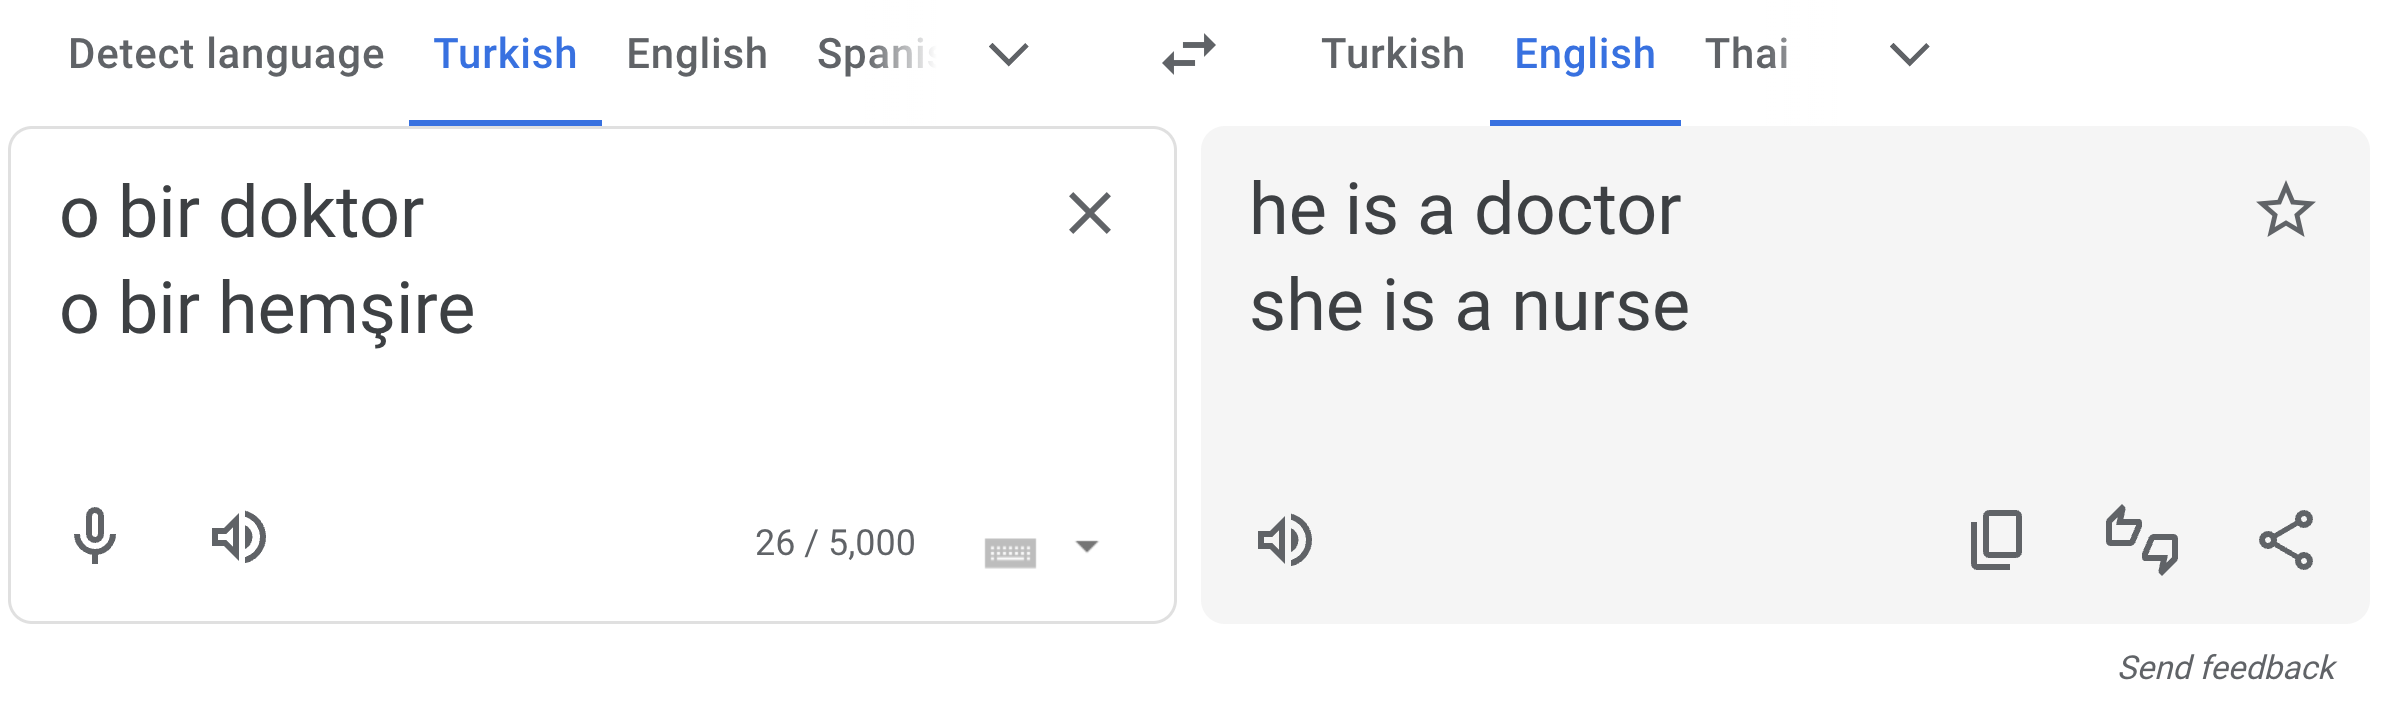
\includegraphics[width=0.9\textwidth]{sections/background/turkish-to-eng.png}
  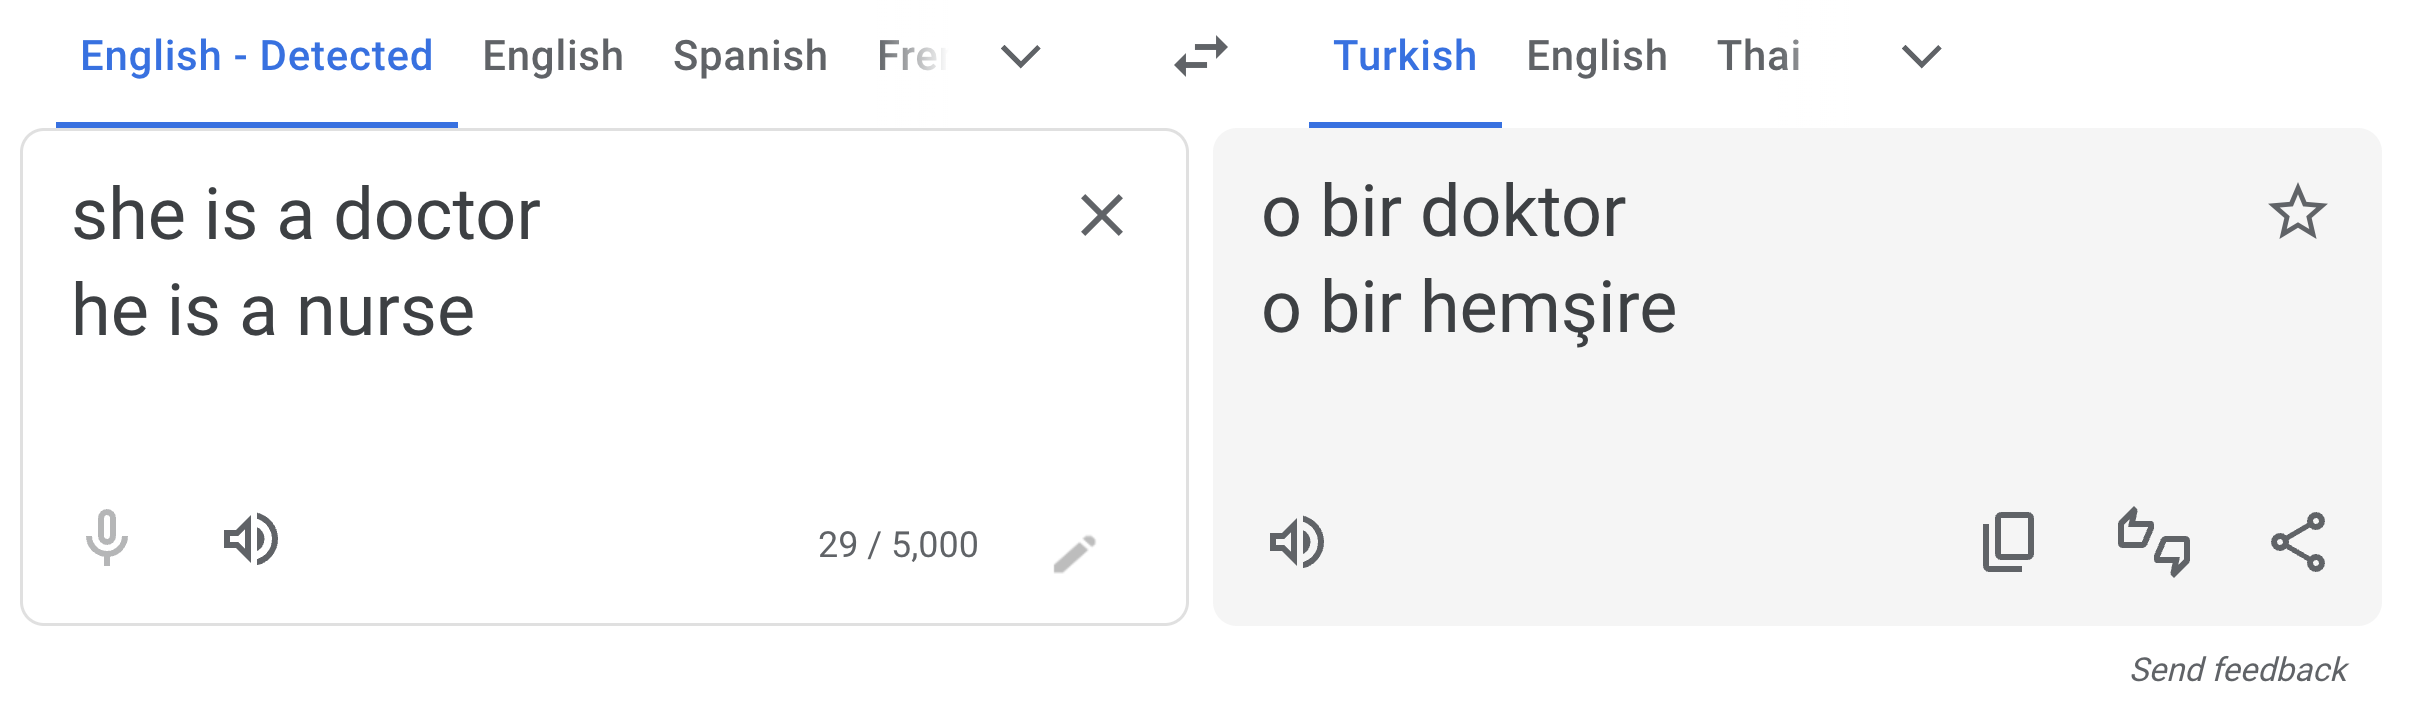
\includegraphics[width=0.9\textwidth]{sections/background/eng-to-turkish.png}
  \caption{Translations of gender-specific English sentences into
  gender-neutral Turkish and then back to English.}
  \label{fig:eng-to-turkish}
\end{figure}

Attempts to mitigate biases by removing explicitly sensitive
attributes (such as gender or race) from training datasets frequently
fall short due to \textit{proxy variables}. Proxy attributes—such as
the age at which individuals start programming—can inadvertently
encode sensitive information like gender, reinforcing biases even in
their absence. Additionally, biases due to disparities in sample
sizes among demographic groups lead to poorer model performance for
minority groups, reinforcing systematic inequities~\cite{barocas2016big}.

Beyond technical considerations, fairness intersects profoundly with
ethical and legal imperatives. Legal frameworks such as Title VII of
the U.S. Civil Rights Act mandate nondiscrimination in employment.
Similarly, regulatory initiatives like the European Union’s GDPR and
proposed AI Act embed fairness, transparency, and equity into
regulatory requirements for algorithmic systems.

Ethically, ensuring fairness aligns closely with broader principles
of justice and equity, particularly as algorithmic systems
increasingly influence societal outcomes such as employment,
education, and criminal justice. Effective fairness interventions
help prevent reinforcing historical injustices, foster social equity,
and maintain public trust in algorithm-driven decision-making.

\subsection{Challenges, Limitations, and Future
Directions}\label{subsec:challenges_future}
(TODO: citations here need to be filled in carefully I relied a bit
on yt tAjFuhkiV2c)

The growing emphasis on fairness in algorithmic decision-making,
particularly in clustering and machine learning contexts, has
significantly advanced our understanding of bias mitigation.
Nevertheless, this field continues to face considerable challenges
and inherent limitations.

One prominent difficulty arises from conflicting fairness criteria.
It is mathematically impossible to simultaneously satisfy all
fairness definitions—such as Demographic Parity, Equal Opportunity,
and Equalized Odds—highlighting the necessity for context-specific
fairness solutions. For example, attempts to apply broad fairness
concepts, initially developed within supervised learning frameworks,
to clustering tasks often encounter mismatches in meaning. Individual
fairness definitions emphasizing distributional equity may not
translate effectively into clustering contexts, where groups or
clusters often lack inherent meaning until assigned. This mismatch
underscores the need to carefully adapt fairness criteria from
supervised learning to unsupervised scenarios.

Moreover, algorithmic fairness interventions rarely function in
isolation. They typically constitute components within broader
socio-technical systems, necessitating careful consideration of both
upstream inputs and downstream impacts. The removal of sensitive
variables, a common fairness strategy, can inadvertently lead to
unintended consequences. For instance, the practice of "Ban the Box,"
intended to eliminate employment discrimination by prohibiting
questions about criminal history, inadvertently increased racial
discrimination as employers began using race as a proxy variable.
This underscores the complexity and potential pitfalls inherent in
algorithmic fairness interventions and highlights the importance of
anticipating and managing unintended downstream consequences.

Further complications emerge from the dynamic nature of real-world
data. In applications such as school districting or political
redistricting, clustering algorithms are applied to dynamic
populations, where individuals may relocate in response to
algorithmic interventions. Historical efforts like school busing
aimed at integrating racially segregated districts illustrate how
algorithmic clustering solutions can unintentionally disrupt
communities or exacerbate segregation through mechanisms such as
"white flight." This historical context reveals the critical need to
engage deeply with domain-specific constraints, legal frameworks, and
stakeholder needs, reinforcing that algorithmic solutions must be
cognizant of broader historical and societal dynamics.

Indeed, addressing these multidimensional challenges requires
interdisciplinary collaboration beyond computer science. Integrating
insights from fields such as sociology, criminology, economics, law,
and ethics is critical. For instance, fairness research often
overlooks valuable contributions from disciplines like criminology or
education policy, which provide nuanced understandings of systemic
inequities and practical constraints. Collaboration with experts from
these domains can guide the appropriate adaptation of algorithmic
methods to complex social contexts, ensuring solutions align closely
with practical realities and ethical standards.

Another essential consideration is stakeholder engagement. Too often,
fairness solutions are developed paternalistically, without
adequately involving those directly impacted. Engaging
stakeholders—including affected communities, policy experts, and
practitioners—in defining fairness and assessing interventions can
prevent misguided assumptions and ensure that algorithmic systems
genuinely serve intended beneficiaries. This is particularly evident
in sensitive domains such as criminal justice, healthcare, and
education, where the risk of inadvertently causing harm or
perpetuating injustices remains high.

Finally, reliance on commonly used benchmark datasets, such as the
COMPAS, Adult, and German Credit datasets, introduces risks of
replicating inherent data biases and inaccuracies. Issues such as
noisy demographic labels, inappropriate or misleading features, and
the misalignment of fairness labels highlight critical weaknesses in
the existing empirical evaluation landscape. Consequently, rigorous
methodological scrutiny and the development of better benchmarks
reflecting real-world complexities and accurate demographic
information are urgently needed.

In summary, future directions in algorithmic fairness research must
navigate inherent mathematical and practical complexities through
rigorous interdisciplinary collaboration, careful stakeholder
engagement, and meticulous empirical practices. By integrating
technical algorithmic approaches with broader societal, legal, and
ethical considerations, researchers can develop more robust,
equitable, and practically viable solutions to mitigate algorithmic
biases and their profound societal implications.


	\section{Preliminaries and Fairness in Clustering}\label{sec:fair_clustering}
		\subsection{Clustering Algorithms}
A clustering algorithm \(A\) partitions an input dataset \(X \in
\mathbb{R}^{n \times m}\) into \(k\) clusters, where \(k \leq n\).
Formally, the algorithm outputs a set \(C = \{C_1, C_2, \dots,
C_k\}\), with each cluster \(C_i \subseteq X\), such that each data
sample \(x \in X\) is assigned to at least one cluster. Depending on
cluster assignment strategies, clustering is broadly categorized into two types:

\begin{itemize}
  \item \textbf{Hard clustering:} Each data point \(x\) belongs to
    exactly one cluster.
  \item \textbf{Soft clustering:} Data points may belong partially or
    probabilistically to multiple clusters.
\end{itemize}

In clustering tasks, unlike supervised learning, labels for data
samples are unavailable. Consequently, the same dataset \(X\) is used
for both training and evaluating the clustering outcomes. This
complicates the definition and enforcement of fairness, as
conventional fairness measures for supervised methods rely on labels
to evaluate biases or discrimination.

The number of clusters \(k\) can either be provided as an input
parameter or determined by the clustering method itself. For
instance, in \(k\)-means, \(k\) is predefined, whereas hierarchical
clustering outputs a dendrogram without a predetermined \(k\),
allowing users to choose the number of clusters post hoc.

\subsection{Taxonomy of Clustering Methods}
A diverse set of clustering methodologies exists, each employing
distinct strategies and assumptions. Following the taxonomy presented
by Xu et al. \cite{XuSurvey}, we classify clustering algorithms as follows:

\begin{enumerate}

  \item \textbf{Center-Based Clustering:} These algorithms partition
    the data to minimize an error metric between samples and their
    cluster center. The canonical example is \(k\)-means, which
    minimizes the squared Euclidean distance.

  \item \textbf{Hierarchical Clustering:} This approach creates a
    binary tree (dendrogram) where the root node represents the
    entire dataset, leaf nodes represent individual samples, and
    intermediate nodes represent clusters. Hierarchical clustering
    methods are either agglomerative (bottom-up) or divisive
    (top-down). We will specifically take a closer look at
    Hierarchical clustering methods in the following sections.

  \item \textbf{Mixture Model-Based Clustering:} A probabilistic
    approach that assumes data points originate from a mixture of
    underlying distributions. Algorithms in this class, such as
    Gaussian Mixture Models (GMM), optimize parameters to best fit
    the data distribution, typically via Expectation Maximization.

  \item \textbf{Graph-Based Clustering:} Data is first represented as
    a graph, where vertices represent samples, and edges denote
    similarity or proximity between samples. Clustering is performed
    by partitioning the graph based on its spectral properties,
    commonly by using eigenvectors of the Laplacian matrix.
    Graph-based clustering is particularly advantageous in scenarios
    involving complex relational data or non-convex clusters.

  \item \textbf{Fuzzy Clustering:} Unlike traditional clustering,
    fuzzy clustering assigns samples a grade of membership to
    clusters. Fuzzy C-Means (FCM) is the archetypal algorithm, where
    data points have partial cluster memberships, reflecting
    uncertainty or gradual boundaries between clusters.

  \item \textbf{Combinatorial Search-Based Clustering:} Many
    clustering objectives are NP-hard, prompting approaches to
    reformulate the clustering problem as a combinatorial
    optimization task. Evolutionary algorithms, genetic algorithms,
    and simulated annealing are typical techniques used to explore
    solutions efficiently.

\end{enumerate}

\subsection{Fairness in Machine Learning}
As previously discussed in Section~\ref{subsec:algorithmic_bias},
machine learning algorithms can unintentionally perpetuate and
amplify societal biases embedded in historical data. These biases
pose significant ethical and practical challenges, particularly in
high-stakes applications like criminal justice, hiring, or
healthcare. Consequently, considerable research effort has been
dedicated to mitigating bias and ensuring fairness in machine learning models.

Fairness interventions can be applied at different stages of the
machine learning pipeline. Specifically, fairness strategies are
commonly categorized as follows:

\begin{enumerate}
  \item \textbf{Pre-processing}: The original dataset is modified
    prior to training or clustering to ensure fair representation or
    remove biases. This approach directly addresses biases inherent
    in training datasets and biases due to missing or
    underrepresented data, as introduced in
    Section~\ref{subsec:algorithmic_bias}.

  \item \textbf{In-processing}: Fairness constraints are integrated
    directly into the algorithm's learning objective. In-processing
    approaches typically modify optimization criteria or integrate
    fairness considerations into model structures, explicitly
    counteracting optimization biases highlighted in the previous
    discussion of algorithmic bias.

  \item \textbf{Post-processing}: Model outputs or clusters undergo
    modification after the learning or clustering process to meet
    fairness constraints. However, for clustering tasks,
    post-processing methods are less common due to the absence of
    labeled validation sets, as clustering is inherently unsupervised.
\end{enumerate}

Defining and enforcing fairness in unsupervised settings, such as
clustering, is especially challenging. Unlike supervised
learning—where fairness criteria, such as Demographic Parity or
Equalized Odds (Section~\ref{subsec:fairness_definitions}), rely on
labeled outcomes—in clustering, no explicit labels are available.
Thus, clustering fairness typically involves ensuring adequate
representation of protected groups within clusters
(\textit{group-level fairness}), or ensuring that individuals who are
similar according to a defined similarity measure receive similar
clustering outcomes (\textit{individual-level fairness}). These
notions extend the concepts of individual fairness (similar treatment
of similar cases) and group fairness (statistical parity across
demographic groups) discussed in the previous section.

The absence of explicit labels complicates direct application of
standard supervised fairness metrics. Consequently, specialized
fairness notions and metrics tailored explicitly for clustering tasks
have emerged, as detailed in the subsequent section.

\subsection{Fairness Notions for Clustering}
Fairness notions in clustering can be classified into these four categories:

\begin{itemize}
  \item \textbf{Group-Level Fairness}: Inspired by the Disparate
    Impact doctrine, these notions aim to ensure no protected group
    (e.g., based on ethnicity or gender) is disproportionately disadvantaged.
  \item \textbf{Individual-Level Fairness}: Ensures similar
    individuals receive similar clustering outcomes, typically
    defined using a dissimilarity metric.
  \item \textbf{Algorithm Agnostic Notions}: Defined independently of
    the clustering algorithm and applicable universally across
    clustering methods.
  \item \textbf{Algorithm Specific Notions}: Tailored specifically
    for certain clustering objectives or algorithms, such as the
    social fairness cost for \(k\)-means clustering.
\end{itemize}

As we move forward, the following mathematical definitions for prominent
fairness notions in clustering will be important:
[\cite{ChhabraOverview}ChabbraIEEE]

\begin{itemize}

  \item \textbf{Balance:} A cluster solution has a high balance if
    each protected group is proportionally represented in each
    cluster. For \(m\) protected groups, define \(r\) as the
    proportion of samples belonging to protected group \(b\) in the
    dataset and \(r_a\) as the proportion of group \(b\) members in
    cluster \(a\). Then, balance is defined as:
    \[
      \text{Balance} = \min_{a\in [k], b\in [m]}
      \min\left\{\frac{r}{r_a}, \frac{r_a}{r}\right\}
    \]

    Balance takes values between 0 and 1, with higher values
    indicating greater fairness.

  \item \textbf{Bounded Representation:} Enforces constraints on the
    maximum (\(\alpha\)) and minimum (\(\beta\)) proportions of
    protected group members in clusters. For each cluster \(a\) and
    protected group \(b\), the constraint is:
    \[
      \beta \leq P_{a,b} \leq \alpha, \quad \forall a\in [k], b\in [m]
    \]

  \item \textbf{Max Fairness Cost (MFC):} Measures deviation from a
    user-specified ideal proportion \(I_b\) for each protected group
    \(b\). The proportion of group \(b\) points in cluster \(a\) is
    \(P_{a,b}\), and MFC is defined as:
    \[
      \text{MFC} = \max_{a\in [k]} \sum_{b\in [m]} |P_{a,b} - I_b|
    \]

  \item \textbf{Social Fairness Cost:} For a set of cluster centers
    \(U\), the clustering cost for group \(a\) is \(O(U, X_a) =
    \sum_{x \in X_a} \min_{u \in U}\|x - u\|^2\), and the social
    fairness cost is defined as:
    \[
      \text{Social Fairness Cost} = \max_{a \in [m]} \frac{O(U, X_a)}{|X_a|}
    \]

    The objective here is to minimize this cost to ensure equitable
    clustering quality across groups.

  \item \textbf{Distributional Individual Fairness:} Assumes an
    \(f\)-divergence \(H_f(V_x \| V_y)\) measuring statistical
    distance between output distributions \(V_x\) and \(V_y\) of
    samples \(x\) and \(y\). Given a fairness similarity measure
    \(F(x,y)\), fairness requires:
    \[
      H_f(V_x \| V_y) \leq F(x,y), \quad \forall x,y \in X \times X
    \]

  \item \textbf{Kleindessner et al.'s Individual Fairness:} Ensures
    for each sample \(x\), belonging to cluster \(C_a\), the average
    distance \(d\) to samples in its cluster is at most the average
    distance to samples in any other cluster \(C_b\):
    \[
      \frac{1}{|C_a| - 1}\sum_{z \in C_a} d(x,z) \leq
      \frac{1}{|C_b|}\sum_{z \in C_b} d(x,z), \quad \forall b \neq a
    \]

  \item \textbf{Entropy (used mainly in deep clustering models)}:
    Defined based on the representation of each protected group in
    clusters. Let \(N_{a,b}\) denote the set of samples belonging to
    both cluster \(a\) and protected group \(b\), and \(n_a\) the
    total samples in cluster \(a\). Then entropy is defined as:
    \[
      \text{Entropy} = -\sum_{a \in [k]} \frac{|N_{a,b}|}{n_a} \log
      \frac{|N_{a,b}|}{n_a}
    \]

    Higher entropy indicates higher fairness within clusters.

\end{itemize}

Balancing fairness constraints with clustering quality often presents
trade-offs, motivating methods that aim to find \emph{Pareto-optimal}
solutions that best balance these competing objectives~\cite{ChhabraOverview}.


	\section{Hierarchical Clustering and Cost}
		Given the ethical and societal implications of algorithm-driven
decisions, understanding the underlying methodologies is essential.
Among these, hierarchical clustering stands out as an influential
unsupervised learning technique widely applied to discover natural
groupings and reveal intrinsic structures within complex data. Its
flexibility in cases where the number of clusters is unknown
beforehand makes it particularly valuable, adapting to various
analytical contexts.

\subsection{Structure and Representation}\label{subsec:hierarchical_clustering}

Hierarchical clustering organizes a dataset \(X\) into a structured
hierarchy of nested clusters, represented by a tree-like diagram
known as a \textit{dendrogram}. Each leaf node corresponds to an
individual data point, while internal nodes represent clusters formed
through either merging or splitting of points. The dendrogram offers
a multi-resolution view, enabling users to explore and select
clusters at varying degrees of granularity. Unlike flat clustering
methods (e.g., \(k\)-means), hierarchical methods do not require
pre-specification of the number of clusters, providing a flexible
structure adaptable to different analytical needs.

\begin{figure}[h]
  \centering
  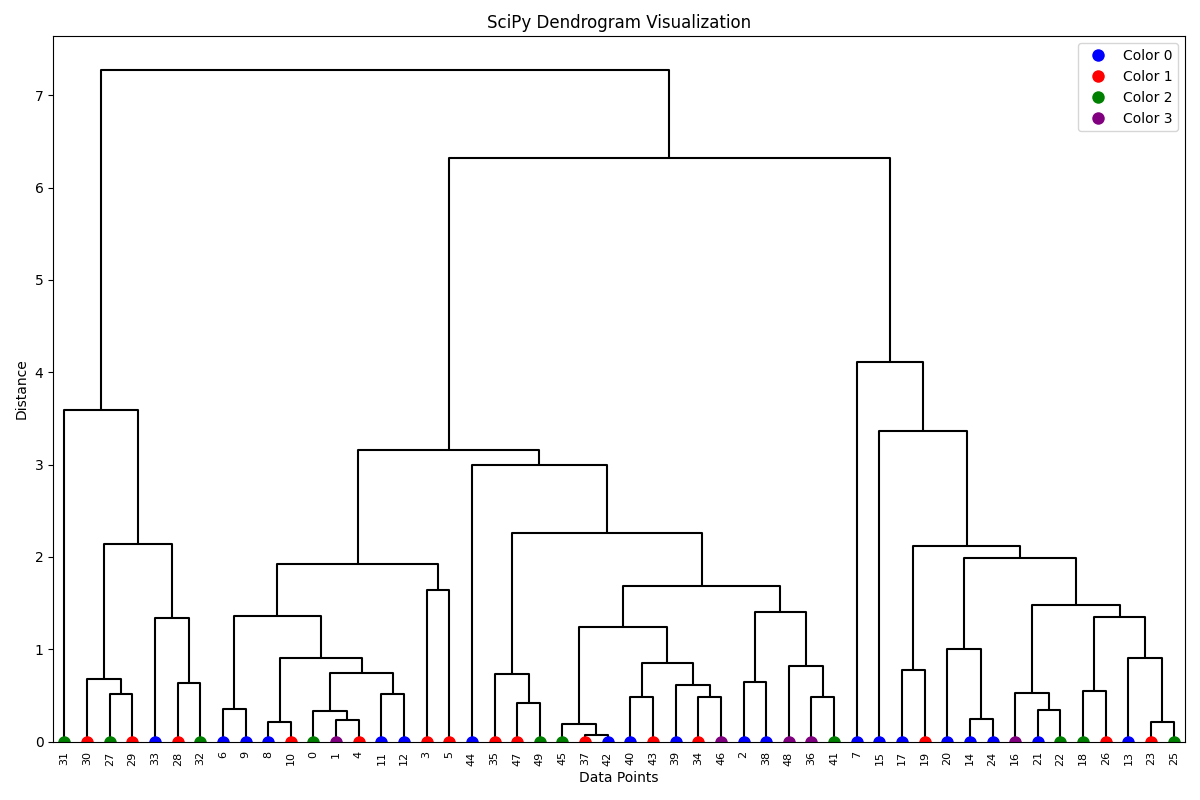
\includegraphics[width=0.9\textwidth]{sections/background/scipy_dendrogram.png}
  \caption{An example of a dendogram representation.}
  \label{fig:example-dendogram}
\end{figure}

Formally, hierarchical clustering constructs a nested partitioning of
a dataset \(X\), such that each cluster at a given resolution is
entirely contained within clusters at coarser resolutions, ensuring
consistency across hierarchical levels.

Hierarchical clustering methods are broadly categorized into two
complementary approaches: \textit{agglomerative} (bottom-up) and
\textit{divisive} (top-down).

\paragraph{Agglomerative Clustering (Bottom-Up Approach).}
Agglomerative hierarchical clustering (AHC) begins with each data
point as a singleton cluster. Clusters are iteratively merged
according to their proximity, defined by a linkage criterion, until
all points form a single cluster. The choice of linkage significantly
impacts the structure and characteristics of resulting clusters.
Some common linkage methods are listed below, however, these are
numerous and the choice of linkage criterion is highly dependent on
the application and underlying data. [SCIPY DOCS HAVE CITS]

\begin{itemize}
  \item \textbf{Single-Linkage:} This method defines the distance
    between two clusters by the shortest distance between any point
    in one cluster and any point in the other. It is known to capture
    irregular cluster shapes but can suffer from a “chaining effect,”
    where clusters may form long, snake-like structures.
    \begin{align*}
      \min_{a \in A, b \in B} d(a, b)
    \end{align*}

  \item \textbf{Complete-Linkage:} This method measures the distance
    between two clusters by looking at the maximum distance between
    any point in one cluster and any point in the other. It typically
    yields compact, roughly spherical clusters, and is robust against
    outliers because it considers the farthest pair of points.
    \begin{align*}
      \max_{a \in A, b \in B} d(a, b)
    \end{align*}

  \item \textbf{Average-Linkage (UPGMA):} In this approach, the
    distance between two clusters is computed as the average distance
    between all pairs of points (one from each cluster). This often
    produces balanced clusters and has widespread empirical success
    across diverse applications.
    \begin{align*}
      \frac{1}{|A| \cdot |B|} \sum_{a \in A} \sum_{b \in B} d(a, b)
    \end{align*}

  \item \textbf{Centroid-Linkage:} This method uses the distance
    between the centroids (mean positions) of two clusters. It forms
    clusters that tend to be spherical, and it has comparatively
    moderate computational requirements.
    \begin{align*}
      \| \mu_A - \mu_B \|^2
      \quad \text{(where $\mu_A$ and $\mu_B$ are centroids of A and B)}
    \end{align*}

  \item \textbf{Ward’s Method:} This approach merges the pair of
    clusters that leads to the smallest increase in the overall
    within-cluster variance (sum of squared distances) at each step.
    Although its mathematical formulation can be quite involved (and
    hence is omitted here), the end result is the creation of cohesive,
    balanced clusters. However, it can be more computationally
    expensive for large datasets.
\end{itemize}

The agglomerative approach's primary advantage lies in its conceptual
simplicity, interpretability, and deterministic nature, but it
typically incurs a computational complexity of \(O(n^2\log n)\) or
\(O(n^3)\), depending on the linkage method and implementation.

\paragraph{Divisive Clustering (Top-Down Approach).}
Divisive hierarchical clustering operates in the reverse direction:
it begins by placing all data points into a single comprehensive
cluster. At each iteration, this cluster is recursively split into
smaller clusters according to a specified criterion—often focusing on
maximizing inter-cluster distance or minimizing intra-cluster
similarity—until each cluster contains only one data point.

Divisive clustering provides a complementary perspective to
agglomerative methods, allowing potentially clearer initial
partitioning of the data. However, divisive algorithms generally
require greater computational resources, as optimal splitting is
typically more computationally intensive than merging clusters. Due
to this increased complexity, divisive clustering is less commonly
used in practice but is valuable in contexts where meaningful
top-level partitions are prioritized.

\subsection{Cost Functions in Hierarchical Clustering}
To quantitatively assess and optimize hierarchical clustering,
researchers have proposed explicit \textbf{cost functions}
\cite{dasgupta2016cost}. These functions take an input graph and a
hierarchical clustering (represented by a tree) and output a value
representing the goodness of the hierarchy.

\paragraph{Dasgupta's cost function} is a formal,
pairwise-similarity-based objective that allows rigorous evaluation
and comparison of hierarchical clustering outcomes
\cite{dasgupta2016cost}. Given a weighted similarity graph
$G=(V,E,w)$, the cost of a hierarchy $T$ is defined as:

\begin{equation*}
  \text{cost}_G(T) = \sum_{e=(x,y) \in E} w(e) \cdot |T_{xy}|
\end{equation*}

where $|T_{xy}|$ is the size of the smallest cluster in $T$
containing both $x$ and $y$. A higher cost indicates that similar
points are clustered loosely in the hierarchy, which is undesirable.
Optimizing Dasgupta's cost function is NP-hard, and the best known
approximation algorithm has a factor of $O(\sqrt{\log n})$.

\paragraph{Mosley's Revenue}
proposed by Moseley and Wang, is defined in the
context of similarity edge weights. It is closely related to cost,
but instead of multiplying the edge weight by the size of the
smallest containing cluster, it uses a related measure. Revenue and
cost are dual to each other, meaning a hierarchy optimizing one also
optimizes the other. Average linkage is a constant-factor
approximation for revenue.

\paragraph{Cohen's Value}
introduced by Cohen-Addad et al.
[\cite{cohen}], is defined in the context where edge
weights represent differences or dissimilarities. The formula for
value is the same as for cost, but because the context of edge
weights is different, it becomes a maximization function. Similar to
revenue, average linkage is a constant-factor approximation for value.

\paragraph{}These cost functions allow for theoretical evaluation of
hierarchical clustering algorithms.

\subsection{Applications of Hierarchical Clustering.}
Hierarchical clustering's flexibility and interpretability have
enabled it to become pervasive across diverse application areas.
Notable examples include:

\paragraph{Computational Biology and Bioinformatics:} Widely
employed for gene expression analysis to discover clusters of
co-expressed genes, thereby elucidating biological pathways and
functions. Additionally, hierarchical clustering underpins the
construction of phylogenetic trees, revealing evolutionary
relationships among species or genetic sequences.

\paragraph{Image Processing and Computer Vision:} Hierarchical
methods are integral to multi-scale image segmentation,
effectively organizing pixels into coherent regions at various
resolutions. Such techniques facilitate detailed scene
understanding, object detection, and content-based image retrieval.

\paragraph{Natural Language Processing (NLP):} Extensively
applied in document clustering to identify thematic groupings,
thereby enabling structured information retrieval, summarization,
and exploration of large textual corpora. Hierarchical clustering
is also instrumental in developing taxonomies and concept
hierarchies in ontology construction.

\paragraph{Marketing and Customer Analytics:} Businesses
frequently utilize hierarchical clustering for market
segmentation and customer profiling, revealing detailed consumer
segments based on purchasing behaviors, demographic attributes,
or online activities. This segmentation allows targeted marketing
and personalized recommendations.

\paragraph{Social Network Analysis:} Hierarchical clustering
aids in detecting community structures within networks, capturing
meaningful groupings such as social circles, influencer
communities, or collaborative groups. These structures can inform
targeted interventions, marketing strategies, or community
detection in online platforms.

\paragraph{Psychology and Sociology:} Researchers leverage
hierarchical clustering for psychometric data analysis and social
behavior pattern identification, uncovering latent constructs and
behavioral archetypes within populations. This facilitates
targeted policy-making, interventions, and sociocultural studies.

\paragraph{Healthcare and Medical Diagnostics:} Hierarchical
methods help classify patients based on symptom profiles or
diagnostic test results, improving patient stratification,
treatment personalization, and clinical decision support systems.

The broad applicability across these domains underscores hierarchical
clustering’s effectiveness in capturing complex structures inherent
to diverse datasets, aligning closely with many practical, societal,
and ethical contexts discussed earlier. Nonetheless, the
computational complexity of hierarchical clustering poses a
persistent challenge, especially with massive datasets.

Given hierarchical clustering’s use in sensitive domains like
healthcare, employment, and criminal justice, ensuring fairness
becomes ethically and practically critical. Integrating explicit
fairness constraints into hierarchical clustering—termed \textit{fair
hierarchical clustering} (FHC)—is thus essential to avoid
perpetuating existing biases.
	
	\subsection{Fair Hierarchical Clustering}\label{subsec:fair_hierarchical_clustering}
		
Given the widespread application of hierarchical clustering in sensitive domains such as healthcare, hiring, criminal justice, and social network analysis, ensuring fairness becomes not only ethically imperative but also practically critical. \emph{Fair hierarchical clustering (FHC)} integrates explicit fairness constraints into hierarchical clustering methods, thereby producing cluster hierarchies that respect fairness at every hierarchical level.

\subsubsection{Problem Formulation}

Formally, fair hierarchical clustering requires that fairness constraints are satisfied at every internal node of the clustering hierarchy, rather than solely at a final partition. Consider a dataset \( X \) partitioned into \( \lambda \) protected groups (e.g., gender, ethnicity). A hierarchical clustering \( T \) is considered \emph{fair} if, for every cluster \( C \) in the hierarchy (excluding singletons), the representation of each protected group within that cluster remains within predefined bounds~\cite{knittel2023generalized}. 

Specifically, given parameters \(\alpha_i\), \(\beta_i\) for each group \( i \in [\lambda] \), cluster \( C \) is fair if the proportion of elements belonging to group \( i \) lies within the range:
\[
\beta_i \leq \frac{|C_i|}{|C|} \leq \alpha_i
\]
where \(|C_i|\) denotes the number of points from group \( i \) within cluster \( C \). A common special case, known as \emph{proportional fairness}, occurs when the group proportions within each cluster precisely reflect their proportions in the overall dataset, typically allowing some small tolerance (slack). For example, if the dataset contains 30\% members of one protected group and 70\% of another, each cluster at every level of the hierarchy must approximately reflect this 30/70 ratio~\cite{knittel2023generalized}. Such recursive enforcement of fairness constraints significantly complicates the hierarchical clustering problem, as decisions at higher levels impose stringent constraints on lower-level cluster splits.

Beyond proportional fairness, researchers have introduced the concept of \emph{relative balance}, which refers to structural or size-based balance in the hierarchy itself. Relative balance ensures clusters at each split are not overly skewed in size, avoiding trivial fairness solutions (e.g., singletons or tiny clusters) and enhancing interpretability. Determining suitable notions of balance (size, depth, or distribution of protected groups) remains an active research question, as balance criteria often conflict with optimizing traditional clustering objectives like Dasgupta’s cost~\cite{knittel2023generalized}.

The integration of fairness into hierarchical clustering introduces considerable theoretical and computational challenges. Ensuring local fairness at each step can conflict with global optimization objectives, such as Dasgupta's cost, often necessitating higher-cost merges to maintain fairness. Furthermore, the combinatorial nature of the problem—searching through an exponentially large space of feasible hierarchies constrained by fairness—amplifies complexity. These difficulties require novel formulations and algorithms explicitly designed to balance fairness and clustering quality.

\emph{(Open question: How can fairness and cluster balance constraints be effectively combined, and what constitutes a suitable balance metric in hierarchical clustering?)}

\subsubsection{Algorithmic Approaches and Advances}

Fair hierarchical clustering is a relatively recent research area. Early pioneering work by Ahmadian et al.~\cite{ahmadian2020fairhc} introduced the first formal definition of fair hierarchical clustering, extending the concept of "fairlets" (small, inherently fair subsets of points) from flat clustering into hierarchical clustering. In their approach, the hierarchy is constructed through modified agglomerative or divisive algorithms that ensure fairness at each intermediate merge or split. While groundbreaking, these initial algorithms had significant limitations, including restrictive assumptions (e.g., two equally sized groups) and relatively weak theoretical guarantees, achieving a cost approximation factor of roughly \( O(n^{5/6}\cdot\text{polylog}(n)) \)~\cite{ahmadian2020fairhc}.

Subsequent research by Knittel et al.~\cite{knittel2023generalized} significantly advanced this area by proposing generalized reduction methods. These methods systematically convert any initial (possibly unfair) hierarchical clustering into a fair and balanced hierarchy with provably small increases in cost. Central to their approach is a collection of carefully defined \emph{tree operators}, such as:

\begin{itemize}
    \item \textbf{Subtree Swap:} Exchanges subtrees or nodes between clusters to improve fairness ratios.
    \item \textbf{Leaf Promotion:} Moves certain leaves higher in the hierarchy to correct fairness imbalances.
    \item \textbf{Bifurcation Adjustment:} Modifies splits to evenly distribute protected groups across branches.
    \item \textbf{Merge/Split Adjustments:} Refines cluster boundaries at different hierarchical levels to maintain fairness.
\end{itemize}

By judiciously applying and scheduling these operators, the generalized reduction approach maintains fairness recursively while closely controlling clustering cost. Remarkably, Knittel et al.’s algorithms provide cost approximation guarantees that are polylogarithmic in \( n \), achieving nearly exponential improvements over earlier methods. Furthermore, their framework accommodates multiple protected groups with arbitrary proportions, significantly generalizing earlier restrictive settings~\cite{knittel2023generalized}.

Current state-of-the-art algorithms for fair hierarchical clustering can thus yield solutions provably within polylogarithmic factors of optimal clustering cost, while ensuring fairness at every hierarchical node. Nonetheless, ongoing research aims to further narrow the approximation gaps and enhance practical usability, since current methods involve intricate multi-phase adjustments.

Empirical evidence from recent studies suggests that enforcing fairness constraints typically induces only modest increases in clustering cost, making fair hierarchical clustering viable for real-world use~\cite{ahmadian2020fairhc,knittel2023generalized}. Still, considerable opportunities remain for refining algorithms, improving computational efficiency, and tailoring these methods for domain-specific constraints.

\emph{(Open question: Can fair hierarchical clustering algorithms be made more computationally efficient and practically scalable, and what domain-specific adjustments could enhance their effectiveness?)}


\chapter*{Conclusion}
         \addcontentsline{toc}{chapter}{Conclusion}
	\chaptermark{Conclusion}
	\markboth{Conclusion}{Conclusion}
	\setcounter{chapter}{4}
	\setcounter{section}{0}
	
Here's a conclusion, demonstrating the use of all that manual incrementing and table of contents adding that has to happen if you use the starred form of the chapter command. The deal is, the chapter command in \LaTeX\ does a lot of things: it increments the chapter counter, it resets the section counter to zero, it puts the name of the chapter into the table of contents and the running headers, and probably some other stuff. 

So, if you remove all that stuff because you don't like it to say ``Chapter 4: Conclusion'', then you have to manually add all the things \LaTeX\ would normally do for you. Maybe someday we'll write a new chapter macro that doesn't add ``Chapter X'' to the beginning of every chapter title.

\section{More info}
And here's some other random info: the first paragraph after a chapter title or section head \emph{shouldn't be} indented, because indents are to tell the reader that you're starting a new paragraph. Since that's obvious after a chapter or section title, proper typesetting doesn't add an indent there. 


%If you feel it necessary to include an appendix, it goes here.
    \appendix
      \chapter{The First Appendix}
      \chapter{The Second Appendix, for Fun}


%This is where endnotes are supposed to go, if you have them.
%I have no idea how endnotes work with LaTeX.

  \backmatter % backmatter makes the index and bibliography appear properly in the t.o.c...

% if you're using bibtex, the next line forces every entry in the bibtex file to be included
% in your bibliography, regardless of whether or not you've cited it in the thesis.
    \nocite{*}

% Rename my bibliography to be called "Works Cited" and not "References" or ``Bibliography''
% \renewcommand{\bibname}{Works Cited}

%    \bibliographystyle{bsts/mla-good} % there are a variety of styles available; 
%  \bibliographystyle{plainnat}
% replace ``plainnat'' with the style of choice. You can refer to files in the bsts or APA 
% subfolder, e.g. 
 \bibliographystyle{APA/apa-good}  % or
 \bibliography{thesis}
 % Comment the above two lines and uncomment the next line to use biblatex-chicago.
 %\printbibliography[heading=bibintoc]

% Finally, an index would go here... but it is also optional.
\end{document}
